\documentclass[]{article}
\usepackage{lmodern}
\usepackage{amssymb,amsmath}
\usepackage{ifxetex,ifluatex}
\usepackage{fixltx2e} % provides \textsubscript
\ifnum 0\ifxetex 1\fi\ifluatex 1\fi=0 % if pdftex
  \usepackage[T1]{fontenc}
  \usepackage[utf8]{inputenc}
\else % if luatex or xelatex
  \usepackage{unicode-math}
  \defaultfontfeatures{Ligatures=TeX,Scale=MatchLowercase}
\fi
% use upquote if available, for straight quotes in verbatim environments
\IfFileExists{upquote.sty}{\usepackage{upquote}}{}
% use microtype if available
\IfFileExists{microtype.sty}{%
\usepackage[]{microtype}
\UseMicrotypeSet[protrusion]{basicmath} % disable protrusion for tt fonts
}{}
\PassOptionsToPackage{hyphens}{url} % url is loaded by hyperref
\usepackage[unicode=true]{hyperref}
\hypersetup{
            pdftitle={Title},
            pdfauthor={Carsten Ersch},
            pdfborder={0 0 0},
            breaklinks=true}
\urlstyle{same}  % don't use monospace font for urls
\usepackage{graphicx,grffile}
\makeatletter
\def\maxwidth{\ifdim\Gin@nat@width>\linewidth\linewidth\else\Gin@nat@width\fi}
\def\maxheight{\ifdim\Gin@nat@height>\textheight\textheight\else\Gin@nat@height\fi}
\makeatother
% Scale images if necessary, so that they will not overflow the page
% margins by default, and it is still possible to overwrite the defaults
% using explicit options in \includegraphics[width, height, ...]{}
\setkeys{Gin}{width=\maxwidth,height=\maxheight,keepaspectratio}
\IfFileExists{parskip.sty}{%
\usepackage{parskip}
}{% else
\setlength{\parindent}{0pt}
\setlength{\parskip}{6pt plus 2pt minus 1pt}
}
\setlength{\emergencystretch}{3em}  % prevent overfull lines
\providecommand{\tightlist}{%
  \setlength{\itemsep}{0pt}\setlength{\parskip}{0pt}}
\setcounter{secnumdepth}{5}
% Redefines (sub)paragraphs to behave more like sections
\ifx\paragraph\undefined\else
\let\oldparagraph\paragraph
\renewcommand{\paragraph}[1]{\oldparagraph{#1}\mbox{}}
\fi
\ifx\subparagraph\undefined\else
\let\oldsubparagraph\subparagraph
\renewcommand{\subparagraph}[1]{\oldsubparagraph{#1}\mbox{}}
\fi

% set default figure placement to htbp
\makeatletter
\def\fps@figure{htbp}
\makeatother


\renewenvironment{abstract}
{\begin{quote}
\noindent \rule{\linewidth}{.5pt}\par{\bfseries \abstractname.}}
{\medskip\noindent \rule{\linewidth}{.5pt}
\end{quote}
}


\title{Title}
\author{Carsten Ersch}
\date{The Fixed Date}

\begin{document}


\begin{titlepage}

\centering


\maketitle
\thispagestyle{empty}


\begin{abstract}
This document has no abstract yet

\end{abstract}

\vfill

% Bottom of the page
  {\footnotesize  Created by Carsten Ersch}
  
	{\footnotesize  Report Created \today\par}
\end{titlepage}

{
\setcounter{tocdepth}{2}
\tableofcontents
}

\pagebreak

Load Packages and functions

Data Processing

\section{Introduction and Background}\label{introduction-and-background}

This is a citation (Dickinson 1999) and an in line citation Dickinson
(1999)

\section{Results}\label{results}

\subsection{A graph}\label{a-graph}

this is a reference to the graph below which is called \ref{fig:fig1}

\begin{figure}[htbp]
\centering
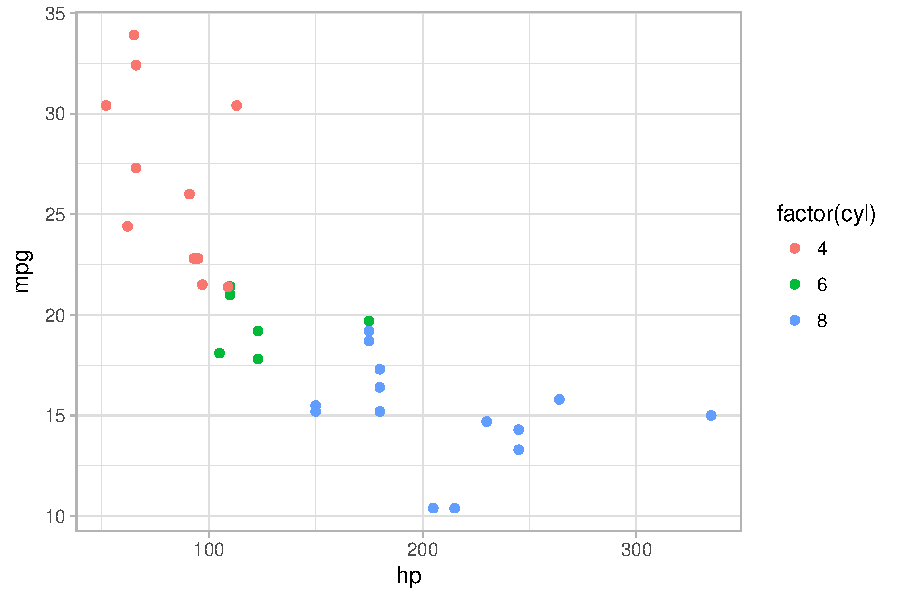
\includegraphics{RMarkdownTemplate_files/figure-latex/fig1-1.pdf}
\caption{\label{fig:fig1} A simple plot}
\end{figure}

\section{Discussion}\label{discussion}

\newpage

\section{Some Basics (to be removed)}\label{some-basics-to-be-removed}

\newpage

\section*{Bibliography}\label{bibliography}
\addcontentsline{toc}{section}{Bibliography}

\hypertarget{refs}{}
\hypertarget{ref-Dickinson1999}{}
Dickinson, Eric. 1999. ``Adsorbed protein layers at fluid interfaces:
Interactions, structure and surface rheology.'' \emph{Colloids and
Surfaces B: Biointerfaces} 15 (2): 161--76.
doi:\href{https://doi.org/10.1016/S0927-7765(99)00042-9}{10.1016/S0927-7765(99)00042-9}.


\end{document}